\section{Experiments}
\label{sec:exp}

\subsection{Setup}
\paragraph{Data.}
\lae \cite{pan2025lae} has 3,592 images and 80 classes taken from the validation sets of FAIR1M \cite{sun2022fair1m}, xView \cite{lam2018xview}, DIOR \cite{li2020dior}, DOTA \cite{xia2018dota} and a power-plant (PP) dataset.
After a logged cleaning step (972 edge boxes clipped, 19 exact duplicates removed) it has 86,539 boxes, and 59\% of them are COCO-small.
Since \lae is a single set, we split it ourselves, once, into dev (730 images) and test (2,862) with iterative multi-label stratification \cite{sechidis2011stratification} (seed 2026), and the ID lists were committed before any detector was run.
All development happened on dev (530 images for calibration, 200 for detection).
The test split was used one time only, with every condition and analysis written down beforehand.
As an external set we use NWPU VHR-10 \cite{cheng2014nwpu}: 614 images and 9 classes mapped to \lae names, with \emph{ship} dropped because it has no single equivalent.

\paragraph{Disjoint label spaces.}
Each source of \lae annotates only its own classes.
A car is ``Small Car'' in FAIR1M, ``Passenger Car'' in xView and ``vehicle'' in DIOR, although the benchmark authors tried to choose classes ``as semantically non-overlapping as possible'' \cite{pan2025lae}.
Under standard COCO evaluation \cite{lin2014coco} a correct ``vehicle'' box on a FAIR1M image is a false positive.
We therefore report \textbf{source-aware} AP (\src), which scores only the classes inside the image's source label space, next to standard AP (\std).
The source is used by the evaluator only, never by the selector.

\paragraph{Metrics and statistics.}
The main metric is AP50 with 900 detections per image; we also report P/R/F1 at score thresholds fixed on dev.
Differences come from a paired image-level bootstrap with 1,000 resamples \cite{efron1993bootstrap}.
For class-averaged AP the percentile interval turned out to be biased (classes drop out of resamples), so we call a difference \emph{robust} only if the percentile CI, the basic CI and a per-class sign test ($p<0.05$, same direction) all agree.
The OVD papers we reviewed mostly report one number per setting, so we felt this extra care was needed for the small absolute values we deal with.

\paragraph{Implementation.}
We use the HF \texttt{transformers} \gdino-T (Swin-T \cite{liu2021swin}, 172M parameters) in fp32 at an 800\,px short side, and \texttt{open\_clip} RemoteCLIP and OpenAI CLIP ViT-B/32.
All checkpoints are pinned by commit hash and sha256.
Detection ran on one RTX 5060 Laptop GPU (8\,GB).
Selection scores are computed once on CPU and saved, so every run uses identical vocabularies.

\subsection{How much headroom is there?}
\label{sec:exp_headroom}
On the 200 dev detection images, giving \gdino all 80 classes yields an AP50 of 0.015 (\std) and 0.028 (\src).
An oracle that gives only the classes present in each image (2.2 classes on average) reaches 0.140, whereas a random list of the same size gets 0.007 / 0.008.
So it is the \emph{content} of the vocabulary that matters, not its length.
An oracle that gives the full label list of the image's source dataset (about 21 classes) reaches only 0.031, which tells us that the selection really has to be made per image.
About 89\% of the oracle gap survives source-aware scoring, so the gap is mostly about per-image relevance and not an artefact of the evaluation.

\subsection{Development results}
\label{sec:exp_dev}
% AA: this table is dev only (200 imgs) and it was used to pick the method, so the numbers are optimistic. we say this in text
\begin{table}[t]
  \centering
  \small
  \begin{tabular}{@{}lccc@{}}
    \toprule
    Selector (dev) & \#cls & AP50 \std & AP50 \src \\
    \midrule
    All 80 classes & 80 & 0.015 & 0.028 \\
    VocAda-style caption top-8 & 8 & 0.022 & 0.034 \\
    TagCLIP-style top-8 & 8 & 0.023 & 0.053 \\
    OpenAI CLIP top-20 & 20 & 0.018 & 0.049 \\
    RemoteCLIP top-8 & 8 & 0.035 & 0.058 \\
    RemoteCLIP + 13 crops, top-8 & 8 & 0.035 & 0.053 \\
    Uncertainty retention & 8.0 & 0.033 & 0.046 \\
    Adaptive top-$p$ & 7.9 & 0.041 & 0.065 \\
    Synonym expansion & 7.6 & 0.052 & \textbf{0.071} \\
    \textbf{Ours (adaptive threshold)} & 7.8 & \textbf{0.055} & \textbf{0.071} \\
    \midrule
    \textit{Oracle (GT classes)} & 2.2 & 0.140 & 0.140 \\
    \bottomrule
  \end{tabular}
  \caption{Development results on 200 dev images. Our rule was picked among 9 rule/size settings on these same images and then frozen, so these numbers are optimistic; \cref{tab:test} is the unbiased result.}
  \label{tab:dev}
\end{table}

\begin{figure}[t]
  \centering
  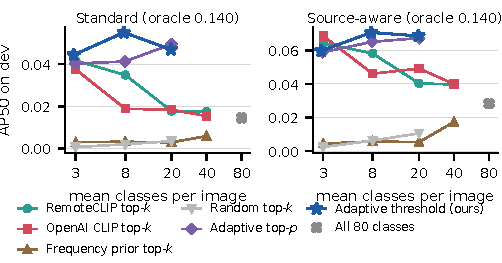
\includegraphics[width=\linewidth]{fig/dev_size_curve.pdf}
  \caption{Dev AP50 against the mean vocabulary size. Fixed top-$k$ selectors with CLIP encoders get worse as $k$ grows, the frequency prior and random lists stay near zero, and the adaptive rules (plotted at their mean size) are best at budgets of 8 and 20 classes.}
  \label{fig:devcurve}
\end{figure}

\cref{tab:dev} summarises the development stage and \cref{fig:devcurve} shows the effect of the budget.
For a fixed top-$k$, smaller is better: RemoteCLIP top-$k$ drops from 0.042 (\std) at $k=3$ to 0.018 at $k=20$, which agrees with the VocAda finding that more classes per noun reduce the gain \cite{liu2025vocada}.
At budgets of 8 and 20 classes the adaptive threshold is better than every fixed $k$ under both protocols, because it can spend a long prompt on an ambiguous image and a one-word prompt on a clear one; at a budget of 3 the fixed selectors are about as good.
OpenAI CLIP and RemoteCLIP are close at most fixed budgets, and RemoteCLIP is clearly ahead only at $k=8$.

The extensions were disappointing.
Local crop evidence improved the \emph{selection} of small-object classes (their recall at $k=8$ went from 0.22 to 0.31) but it did not improve detection: small-object recall went up while small-object AP went down, and the crops cost 83\,ms per image instead of 8\,ms.
Uncertainty retention showed the same pattern.
The caption selector cost about 1.2\,s per image on our GPU, more than three times the detector forward pass, and lost on class-averaged AP.
It won only on pooled F1, because captions often mention cars, which are the densest classes.
Synonym expansion tied on \src and lost on \std, so it failed the replacement rule we had fixed in advance and we kept the simpler method.

\subsection{Main result on the held-out test split}
\label{sec:exp_test}
\begin{table}[t]
  \centering
  \small
  \setlength{\tabcolsep}{4pt}
  \begin{tabular}{@{}lcccc@{}}
    \toprule
    Selector (test) & \#cls & AP50 \std & AP50 \src & vs.\ ours \\
    \midrule
    All 80 classes & 80 & 0.0053 & 0.0157 & robust \\
    Random (oracle size) & 2.3 & 0.0023 & 0.0038 & robust \\
    Frequency prior top-8 & 8 & 0.0028 & 0.0056 & robust \\
    OpenAI CLIP top-20 & 20 & 0.0081 & 0.0238 & robust (\std) \\
    RemoteCLIP top-8 & 8 & 0.0170 & 0.0347 & robust \\
    Adaptive threshold, $\sim$20 & 19.8 & 0.0209 & 0.0378 & n.s. \\
    Adaptive top-$p$, $\sim$20 & 19.8 & 0.0276 & 0.0406 & n.s. \\
    \textbf{Ours, $\sim$8} & 8.0 & \textbf{0.0280} & \textbf{0.0418} & -- \\
    \midrule
    \textit{Oracle} & 2.3 & 0.1072 & 0.1072 & -- \\
    \bottomrule
  \end{tabular}
  \caption{Results on the 2,862 held-out test images (single run, all settings frozen). ``robust'' means ours is better and all three checks agree under both protocols unless noted; n.s.\ = not significant.}
  \label{tab:test}
\end{table}

\cref{tab:test} is our main result.
Compared with the full vocabulary, the selector improves AP50 by +0.0228 under \std (basic CI $[+0.0143, +0.0263]$, 56 classes better against 18 worse, $p=1.1\times10^{-5}$) and by +0.0261 under \src (basic CI $[+0.0163, +0.0300]$, 50 against 24, $p=0.0034$).
The claim we declared before the run therefore holds under both protocols.
This is 22\% (\std) and 29\% (\src) of the oracle headroom.
On dev it was 38\%, so, as expected, the gain shrank somewhat once we stopped choosing the method on the same images.

For us the more interesting comparison is with RemoteCLIP top-8, which uses the \emph{same} encoder and the same average size.
Ours is robustly better under both protocols (+0.011 \std with 50/20 classes; +0.007 \src with 44/26), so the adaptive size really helps and the gain is not just a shorter prompt.
On dev this comparison had passed only two of the three checks, so the test set settled it.
The adaptive top-$p$ rule at about 20 classes is statistically tied with ours, which suggests that the per-image adaptation matters more than the exact budget.

\paragraph{F1.}
At the thresholds fixed on dev, F1 goes from 0.014 to 0.036 (\std) and from 0.039 to 0.056 (\src).
We should also report an awkward result for the metric: the frequency prior reaches a higher pooled F1 (0.084 / 0.132) while having almost the lowest AP.
Its fixed list is mostly FAIR1M vehicle classes plus xView ``Building'', which are the densest classes in the test split, and pooled F1 counts boxes while AP averages over classes.
We keep class-averaged AP as the headline, as declared before the run.

\begin{table}[t]
  \centering
  \small
  \setlength{\tabcolsep}{3.6pt}
  \begin{tabular}{@{}lcccccc@{}}
    \toprule
    & \multicolumn{3}{c}{AP50 \std} & \multicolumn{3}{c}{Recall@IoU0.5} \\
    \cmidrule(lr){2-4}\cmidrule(lr){5-7}
    Test, by object size & S & M & L & S & M & L \\
    \midrule
    All 80 classes & 0.002 & 0.005 & 0.011 & 0.05 & 0.21 & 0.47 \\
    RemoteCLIP top-8 & 0.004 & 0.014 & 0.037 & 0.08 & 0.25 & 0.50 \\
    \textbf{Ours} & \textbf{0.006} & \textbf{0.027} & \textbf{0.063} & \textbf{0.10} & \textbf{0.28} & \textbf{0.54} \\
    \midrule
    \textit{Oracle} & 0.052 & 0.129 & 0.197 & 0.41 & 0.67 & 0.88 \\
    \bottomrule
  \end{tabular}
  \caption{Test results by COCO object size (S $<32^2$, M $<96^2$ px, L otherwise). Selection helps every size, but small objects stay almost 10$\times$ below the oracle.}
  \label{tab:size}
\end{table}

\paragraph{Object size.}
\cref{tab:size} splits the test result by object size.
The relative gain is largest for medium and large objects (AP50 $\times$6.0 and $\times$5.9).
Small objects also improve, but they stay close to zero (0.006 against 0.052 for the oracle).
A tiling diagnostic on dev ($2{\times}2$ tiles plus the full image) did not raise small-object AP, lowered the overall AP of both the oracle (0.140 $\rightarrow$ 0.114) and our method (0.055 $\rightarrow$ 0.039), and was 5$\times$ slower, so we did not pursue it.

\subsection{Where does it work?}
\label{sec:exp_where}
\begin{figure*}[t]
  \centering
  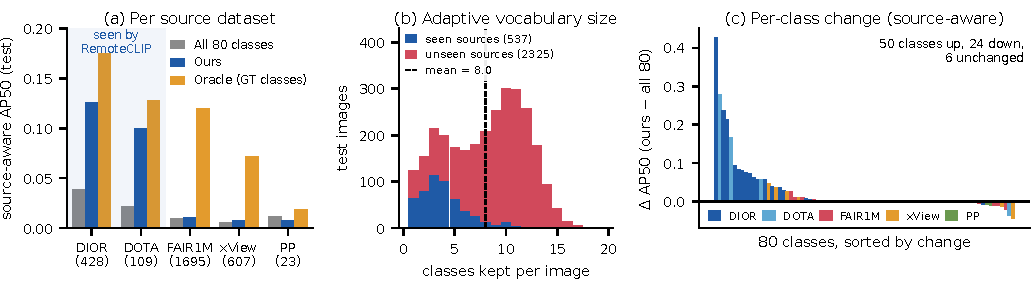
\includegraphics[width=\textwidth]{fig/test_analysis.pdf}
  \caption{Test-split analysis. (a) Source-aware AP50 per source dataset (number of test images in brackets); DIOR and DOTA are in RemoteCLIP's training data. (b) Number of classes kept per image by our frozen rule: images from the seen sources usually keep 1--7 classes, while FAIR1M/xView/PP images keep more. (c) Change in per-class AP50 against the full vocabulary, sorted and coloured by the source of the class.}
  \label{fig:test}
\end{figure*}

RemoteCLIP's training data contains DIOR and DOTA but not FAIR1M or xView \cite{liu2024remoteclip}, so before the test run we fixed a split of \lae sources into a seen group (DIOR, DOTA) and an unseen group (FAIR1M, xView, PP).
\cref{fig:test}a shows that the gain is almost entirely on the seen group: source-aware AP50 rises from 0.035 to 0.120 there (3.5$\times$; 20 of 23 classes better, $p=5\times10^{-4}$), whereas on the unseen group it moves from 0.008 to 0.009 (not significant) although the oracle shows about 11$\times$ headroom.
The vocabulary sizes in \cref{fig:test}b tell the same story from the selector's side.
On seen sources RemoteCLIP is confident and keeps 4.0 classes on average (27\% of these images keep one or two), while on unseen sources it spreads its probability and keeps 8.9.
The per-class view (\cref{fig:test}c) is consistent: the large gains are DIOR and DOTA classes, the FAIR1M and xView classes cluster around zero, and the 24 classes that lose, lose very little.

\begin{table}[t]
  \centering
  \small
  \setlength{\tabcolsep}{4pt}
  \begin{tabular}{@{}lccc@{}}
    \toprule
    NWPU VHR-10 (614 images) & \#cls & AP50 & $\Delta$ vs.\ all 80 \\
    \midrule
    All 80 classes & 80 & 0.088 & -- \\
    RemoteCLIP top-8 & 8 & 0.093 & +0.005 (n.s.) \\
    OpenAI CLIP top-20 & 20 & 0.100 & +0.012 (robust) \\
    \textbf{Ours (frozen $t$)} & 3.9 & \textbf{0.129} & \textbf{+0.041} (robust) \\
    \midrule
    \textit{Oracle} & 1.4 & 0.208 & +0.120 \\
    \bottomrule
  \end{tabular}
  \caption{Transfer to NWPU VHR-10 with every method frozen and no recalibration. Standard and source-aware AP are identical here.}
  \label{tab:nwpu}
\end{table}

\paragraph{External data.}
On NWPU VHR-10, applied without any retuning, our selector improves AP50 from 0.088 to 0.129 (+0.041, CI $[+0.030, +0.057]$, 8 of 9 classes better), while fixed-size RemoteCLIP top-8 gives no significant gain (\cref{tab:nwpu}).
The frozen threshold keeps only 3.9 classes per image here, because RemoteCLIP is more confident on these DIOR-like images, and this is exactly where a fixed $k$ cannot follow.
Most of the gain comes from two classes, ground track field (0.007 $\rightarrow$ 0.243) and vehicle (0.000 $\rightarrow$ 0.163), while airplane, which the full prompt already detects, loses 0.07.
We want to be careful about what this shows.
NWPU was made by the same group as DIOR with DIOR's class names, and LAE-1M even includes it as a training source \cite{pan2025lae}.
So this is transfer to new images of a \emph{familiar} kind, not a general unseen-domain result.
We also could not check image overlap between NWPU and the DIOR training images that RemoteCLIP used.

\subsection{Speed}
On the RTX 5060 (GPU idle, fp32, 200 dev images, 3 passes, selector and detector in the same process) the median end-to-end time is 414\,ms with all 80 classes and 343\,ms with ours, including 7.9\,ms for the selector.
That is 1.21$\times$ faster (difference $-71$\,ms, CI $[-72, -71]$), and peak GPU memory also drops from 2.77 to 2.49\,GB.
The saving comes from the detector itself (414 $\rightarrow$ 335\,ms), as a shorter prompt means less text in the fusion layers, which is related to the cost of long prompts that WeDetect describes for fusion detectors \cite{fu2026wedetect}.
For reference, VocAda reports 5.6--10.7\,s per image on a V100 \cite{liu2025vocada}, but with a different detector, so it is not a direct comparison.

\subsection{Failure analysis}
\label{sec:exp_fail}
\begin{figure*}[t]
  \centering
  \begin{subfigure}{0.325\textwidth}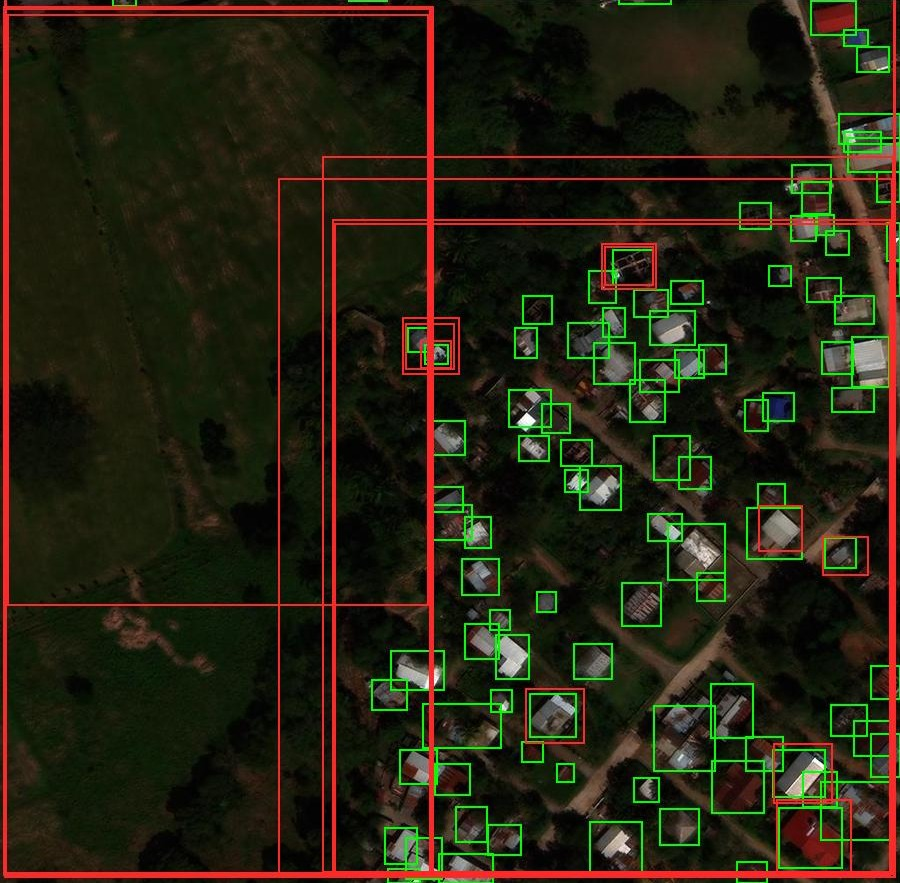
\includegraphics[width=\linewidth]{fig/qual_full.jpg}\caption{All 80 classes}\end{subfigure}\hfill
  \begin{subfigure}{0.325\textwidth}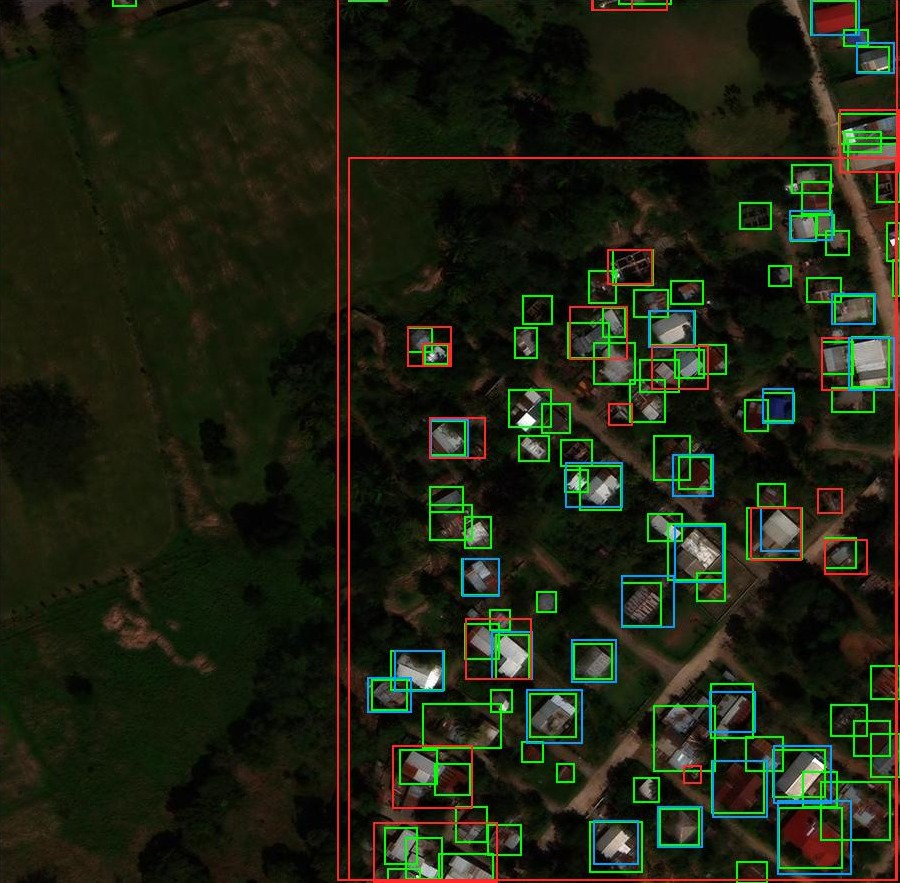
\includegraphics[width=\linewidth]{fig/qual_ours.jpg}\caption{Ours, same image}\end{subfigure}\hfill
  \begin{subfigure}{0.325\textwidth}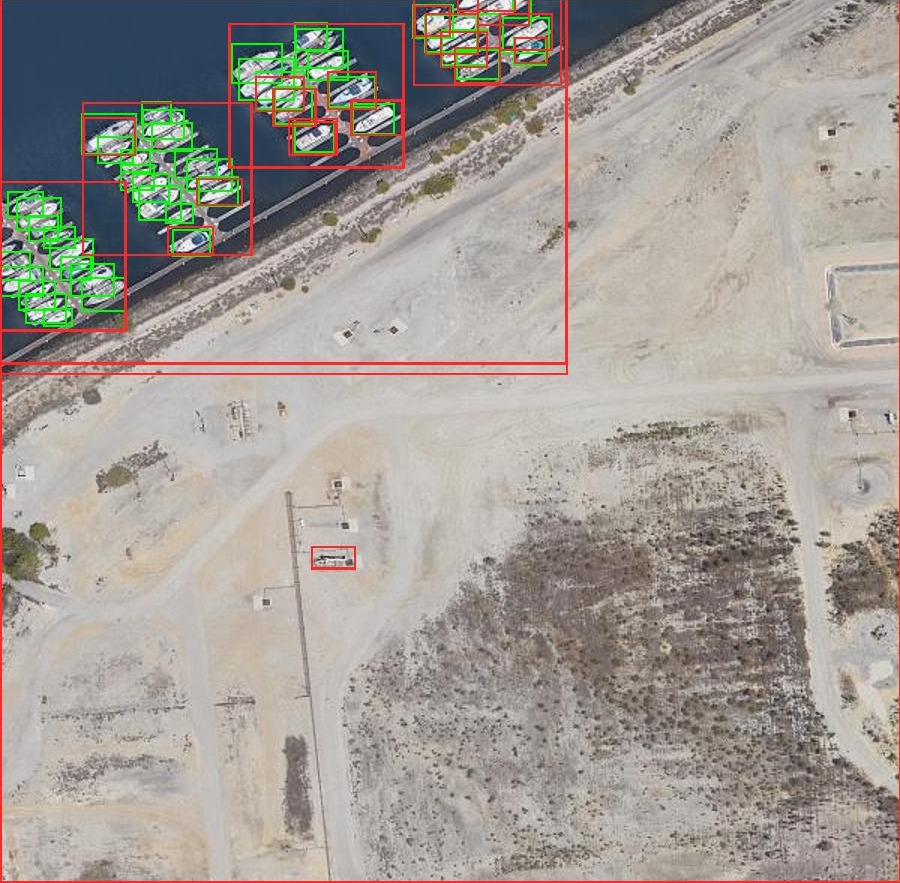
\includegraphics[width=\linewidth]{fig/qual_fail.jpg}\caption{Failure: near-synonym classes}\end{subfigure}
  \caption{Qualitative results on dev images, chosen by fixed rules and not by hand. (a, b) xView village (image 3229), the image with the largest true-positive gain of ours over the full prompt: the full prompt produces huge false boxes, our vocabulary recovers many buildings. (c) FAIR1M marina (image 2154), the image with the most wrong-class outcomes for our method: the boats are boxed well but receive a different class name. Green = ground truth, blue = true positive, red = false positive at score $\geq0.14$.}
  \label{fig:qual}
\end{figure*}

We sorted every labelled object and every confident detection on the dev images into failure types that we had defined before looking at them.
The main findings are listed below, and \cref{fig:qual} shows one success and one failure.
\begin{itemize}
  \item Our selector keeps the right class for only 26\% of ground-truth \emph{objects}, because images with more than 20 objects hold 85\% of all objects, and on FAIR1M and xView it keeps the right class for only 22\% and 24\% of the objects.
  \item 59\% of the selected classes belong to another source's label set, \eg xView ``Ferry'' on a FAIR1M image labelled ``Passenger Ship''. This is the hard-negative problem of \cite{bianchi2024devil} and the overlapping-concept problem of \cite{li2024lbp}, here produced by the benchmark taxonomy. A diagnostic that restricts the selection to the true source raises object coverage from 0.25 to 0.68, but it needs the source label, which a deployable selector does not have.
  \item When the right class \emph{is} kept, \gdino finds 48\% of those objects, against 58\% with the oracle, so in that case the detector behaves almost as if it had the perfect vocabulary.
  \item Confident detections drop by 76\% (28,580 $\rightarrow$ 6,747) and their true-positive share triples (0.008 $\rightarrow$ 0.027). With all 80 classes, 77\% of the confident detections are classes never annotated in that image's dataset.
  \item Selection helps sparse scenes (1--5 objects: 0.025 $\rightarrow$ 0.109 AP50) but hurts scenes with more than 20 objects (0.038 $\rightarrow$ 0.017 for 21--100 objects).
  \item Rare classes stay near zero for every vocabulary, the oracle included (0.050), so better selection cannot rescue them.
\end{itemize}
